%TeX

\section{Reversing the MBR}

\begin{frame}{RE400 what?\ldots}
    \begin{columns}
        \column{0.5\textwidth}
	        \begin{itemize}
                \item Challenge worth 400 points
                \item Reverse Engineering category
                \item We get some hints right away\ldots
                \begin{itemize}
                	\item This is an MBR
                	\item \ldots from an x86 system
        	    \end{itemize}
            \end{itemize}
        \column{0.5\textwidth}
                {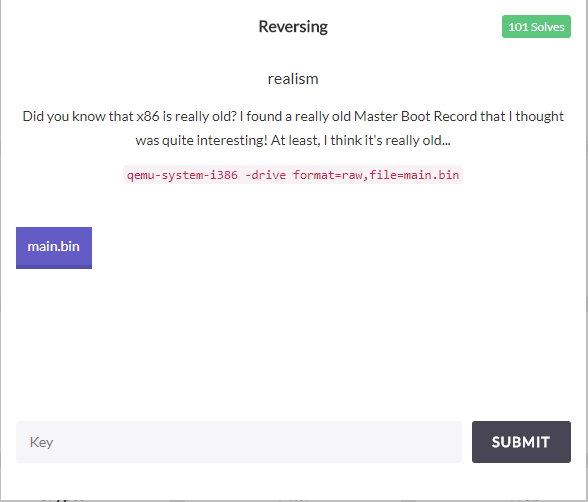
\includegraphics[width=\textwidth]{re400}}
    \end{columns}
\end{frame}

\begin{frame}{A place to start\ldots}
    \begin{columns}
        \column{0.5\textwidth}
	        \begin{itemize}
                \item<1-> Wikipedia, of course!
		        \begin{itemize}
    	            \item<2-> 512 bytes
        	        \item<2-> MBR signature: 55 AA
            	    \item<2-> "expected to contain real mode machine language instructions"
                	\item<2-> little-endian
                	\item<2-> loads at 0000:7C00
	            \end{itemize}                	
            \end{itemize}
        \column{0.5\textwidth}
                {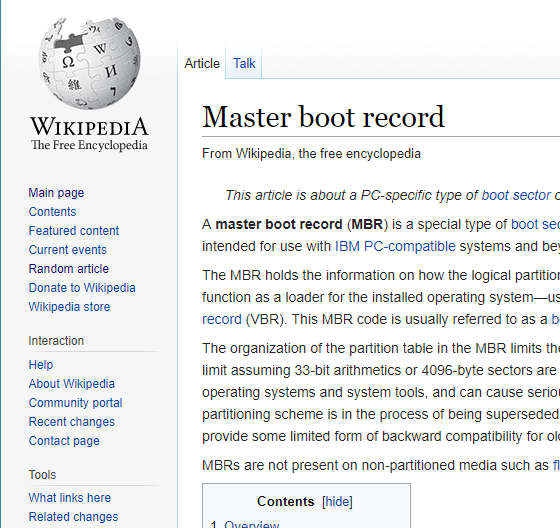
\includegraphics[width=\textwidth]{wikimbr}}
    \end{columns}
\end{frame}

\begin{frame}{Tool Time!\ldots}
    \begin{columns}
        \column{0.5\textwidth}
	        \begin{itemize}
		        \item qemu (gift wrapped)
                \only<1> {
                	\begin{itemize}
                		\item -s (gdb)
            	    	\item -S (suspend)
        	        	\item -vnc:1
	                \end{itemize}
                }
                \only<2> {
                	\begin{itemize}
               			\item QEMU/Monitor
                		\begin{itemize}
	    	            	\item info registers
    	    	        	\item system reset
    	    	        \end{itemize}
        	    	\end{itemize}
        	    }
       	    \end{itemize}
        \column{0.5\textwidth}
                \only<1>{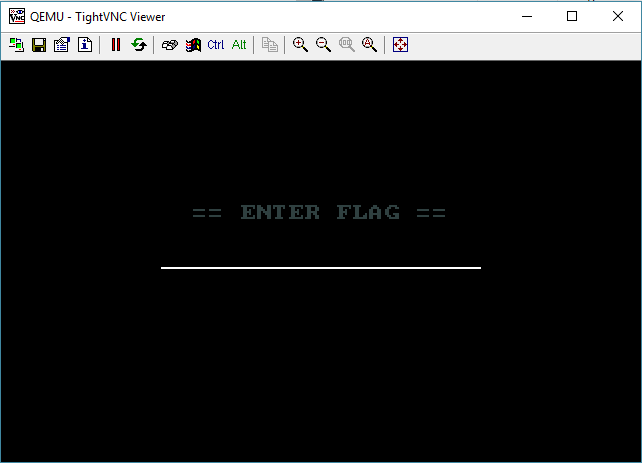
\includegraphics[width=\textwidth]{qemu-vnc}}
                \only<2>{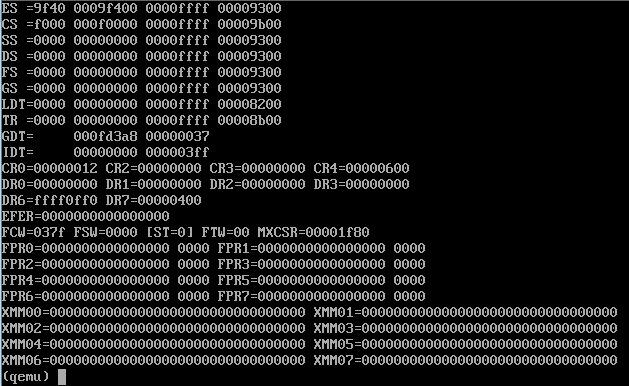
\includegraphics[width=\textwidth]{qemu-info-registers-1}}
    \end{columns}
\end{frame}